\documentclass[12pt]{article}
% \usepackage[czech]{babel}
\usepackage{natbib}
\usepackage{url}
\usepackage{amsmath}
\usepackage{graphicx}
\graphicspath{{images/}}
\usepackage{parskip}
\usepackage{fancyhdr}
\usepackage{vmargin}
\setmarginsrb{3 cm}{2.5 cm}{3 cm}{2.5 cm}{1 cm}{1.5 cm}{1 cm}{1.5 cm}
\usepackage{fancyhdr}
\usepackage{caption}
\usepackage{fixltx2e}
\usepackage{textgreek}
\usepackage{multicol}
\usepackage[hidelinks, colorlinks=true]{hyperref}
\setcitestyle{square}
\setcitestyle{citesep={,}}


							
\makeatletter
\let\thetitle\@title


\makeatother

\pagestyle{fancy}
\fancyhf{}
\rhead{\theauthor}
\lhead{\thetitle}
\cfoot{\thepage}


%%%%%%%%%%%%%%%%%%%%%%%%%%%%%%%%%%%%%%%%%%%%%%%%%%%%%%%%%%%%%%%%%%%%%%%%%%%%%%%%%%%%%%%%%
\begin{titlepage}
	\centering
	\hspace{1 cm}
    
\includegraphics[scale = 0.35]{FIT_logo.png}\\[1.0 cm]	% University Logo
    \hspace{1 cm}
    \textsc{\LARGE BDA project documentation}\\[2.0 cm]
    \hspace{1 cm}
    \textsc{\LARGE Modified ERC20 Token}\\[0.2 cm]

	\quad\rule{15 cm}{0.2 mm}
	{ \huge \bfseries \thetitle}\\
	
	\vspace{1 cm}
	\begin{minipage}{0.45\textwidth}
		
            \newline
			\emph{Author:} \\
			\textbf{Tomáš Beránek (xberan46)} \linebreak\\[2.0 cm]

            
        
	\end{minipage}\\[0 cm]

    \hspace{1 cm}\textbf{\LARGE \href{https://drive.google.com/file/d/1e-1nz6NPWf7WG1fHD7mfNYaYF5ugZXVR/view?usp=sharing}{Demonstration video}}
 
    \vspace{6 cm}
    \begin{flushleft}
   	    E-mail:\hspace{4 cm}\textbf{xberan46@stud.fit.vutbr.cz} \linebreak
        Date:\hspace{4.3 cm}\textbf{May 14th 2023} \linebreak
    \end{flushleft}

	\vfill
    \fancyhf{}
\end{titlepage}


%%%%%%%%%%%%%%%%%%%%%%%%%%%%%%%%%%%%%%%%%%%%%%%%%%%%%%%%%%%%%%%%%%%%%%%%%%%%%%%%%%%%%%%%%


\begin{document}
\afterpage{\cfoot{\thepage }}
\section{ERC20 Token}
\label{erc20}
ERC20 \cite{erc20-blog, erc20-doc} is a technical standard that defines a set of rules and requirements for fungible\footnote{\textbf{fungible tokens} are interchangeable with other tokens of the same type.} tokens on the Ethereum blockchain. It is used to ensure interoperability between tokens and allows them to interact with each other seamlessly. ERC20 tokens are programmable digital assets that can represent various things such as transferable units of value, voting rights, or other functionalities.

The ERC20 standard includes 6 mandatory functions (and 2 events) that all ERC20 tokens must implement:
            
\begin{itemize}
\item \texttt{totalSupply()}
\begin{itemize}
\item[] returns the total number of tokens in circulation,
\end{itemize}
\item \texttt{balanceOf(address owner)}
\begin{itemize}
\item[] returns the balance of \texttt{owner} address,
\end{itemize}
\item \texttt{transfer(address to, uint256 value)}
\begin{itemize}
\item[] transfers \texttt{value} tokens from the sender's address to address \texttt{to},
\end{itemize}
\item \texttt{approve(address spender, uint256 value)}
\begin{itemize}
\item[] allows the \texttt{spender} address to spend up to \texttt{value} tokens on behalf of the sender,
\end{itemize}
\item \texttt{allowance(address owner, address spender)}
\begin{itemize}
\item[] returns the number of tokens that the \texttt{spender} address is allowed to spend on behalf of the \texttt{owner} address,
\end{itemize}
\item \texttt{transferFrom(address from, address to, uint256 value)}
\begin{itemize}
\item[] allows the sender to transfer \texttt{value} tokens from address \texttt{from} to address \texttt{to}, if the sender is authorized to spend the given amount.
\end{itemize}
\end{itemize}

These functions allow for the transfer of tokens between addresses, checking an account's balance, and approving third-party accounts to spend tokens on behalf of the token holder. By following these standards, ERC20 tokens can be easily integrated into decentralized applications (DAPPs) and other projects. They provide a standardized and interoperable way to represent digital assets on the Ethereum blockchain, making it easier to create decentralized applications and exchange value in a transparent and secure manner.

\section{Modified ERC20 Token (BDAERC20)}
\label{next}
The goal of this project is to implement a modified ERC20 token (hereafter referred to as BDAERC20). A list of all modifications is given in the file \texttt{assignment.pdf}. BDAERC20 is implemented in Solidity 0.8.13 and uses the Truffle framework for compilation, testing, deployment, etc.

\begin{figure*}[h]\centering
  \centering
  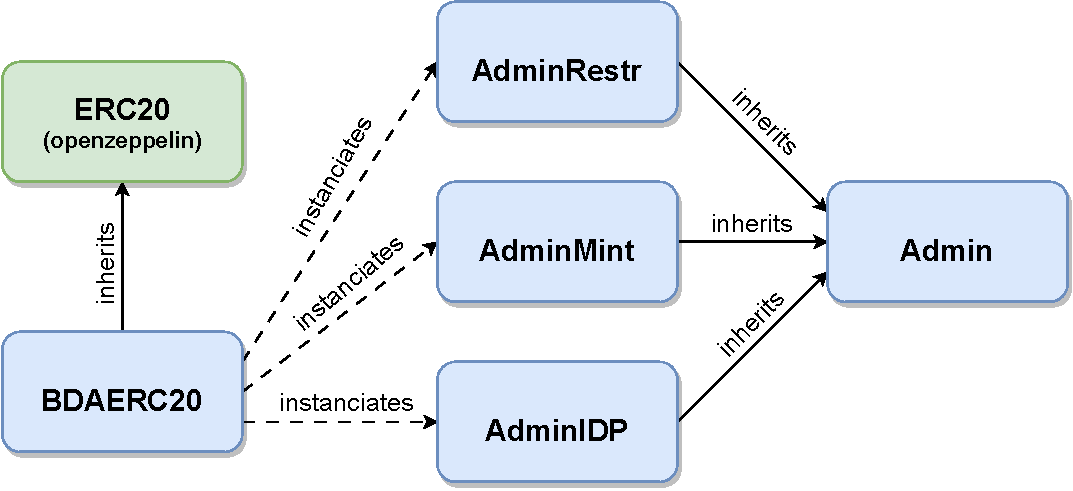
\includegraphics[width=0.8\linewidth]{images/contracts.pdf}
  \caption{Graph of inheritance of implemented contracts. Blue are contracts that have been implemented in the project and green are existing contracts.}
  \label{contracts}
\end{figure*}

The implementation consists of 5 contracts, see Figure \ref{contracts}. The interface for communication with users is the \texttt{BDAERC20} contract, which instantiates contracts for individual admin roles -- \texttt{AdminRestr}, \texttt{AdminMint} and \texttt{AdminIDP}. These admin contracts all inherit from the \texttt{Admin} contract, which provides basic admin account management (store admin addresses, add, remove etc.). \texttt{AdminRestr}, \texttt{AdminMint} and \texttt{AdminIDP} implement admin specific actions. The \texttt{BDAERC20} contract inherits from OpenZeppelin's \texttt{ERC20} \cite{oz-doc} contract, and the \texttt{EnumerableSet} and \texttt{EnumerableMap} libraries also from OpenZeppelin are used as well. In addition to the mandatory and some optional ERC20 functions (see Chapter \ref{erc20}), \texttt{BDAERC20} provides the following functions:

\begin{itemize}
    \item \texttt{isVerified(address user)}
        \begin{itemize}
            \item[] returns information about whether \texttt{user} is verified (returns \texttt{false} when \texttt{user} is revoked),
        \end{itemize}
    \item \texttt{isRevoked(address user)}
        \begin{itemize}
            \item[] returns information about whether \texttt{user} is revoked,
        \end{itemize}
    \item \texttt{isVerifiedUntil(address user)}
        \begin{itemize}
            \item[] returns to which epoch time \texttt{user} is verified,
        \end{itemize}
    \item \texttt{getVerifiedUsers()}
        \begin{itemize}
            \item[] returns a list of verified users,
        \end{itemize}
    \item \texttt{transferedToday(address user)}
        \begin{itemize}
            \item[] returns the number of tokens sent today by the \texttt{user},
        \end{itemize}
    \item \texttt{mint(address$[]$ accounts, uint256$[]$ amounts)}
        \begin{itemize}
            \item[] mint \texttt{accounts} their respective number of \texttt{amounts} tokens,
        \end{itemize}
    \item \texttt{signMint(address$[]$ accounts, uint256$[]$ amounts)}
        \begin{itemize}
            \item[] same as \texttt{mint}, but requires consensus of mint admins and does not count into \texttt{TMAX},
        \end{itemize}
    \item \texttt{signTransferLimitChange(address user, uint256 newValue)}
        \begin{itemize}
            \item[] after restriction admin consensus change daily transfer limit of \texttt{user} to \texttt{newValue},
        \end{itemize}
    \item \texttt{getTransferLimit(address user)}
        \begin{itemize}
            \item[] returns the daily transfer limit of \texttt{user},
        \end{itemize}
    \item \texttt{signTMAXChange(uint newTMAX)}
        \begin{itemize}
            \item[] after mint admin consensus  change \texttt{TMAX} to \texttt{newTMAX},
        \end{itemize}
    \item \texttt{verify(bytes32 hashedMessage, uint8 v, bytes32 r, bytes32 s)}
        \begin{itemize}
            \item[] verifies the sender if the signature is valid and from a valid IDP,
        \end{itemize}
    \item \texttt{getMintContractAddress()}
        \begin{itemize}
            \item[] returns the address of the \texttt{AdminMint} contract (for development purposes),
        \end{itemize}
    \item \texttt{getIDPContractAddress()}
        \begin{itemize}
            \item[] returns the address of the \texttt{AdminIDP} contract (for development purposes),
        \end{itemize}
    \item \texttt{signAddingMintingAdmin(address addr)}
        \begin{itemize}
            \item[] add \texttt{addr} as mint admin after mint admin consensus,
        \end{itemize}
    \item \texttt{signAddingIDPAdmin(address addr)}
        \begin{itemize}
            \item[] add \texttt{addr} as IDP admin after IDP admin consensus,
        \end{itemize}
    \item \texttt{signAddingRestrAdmin(address addr)}
        \begin{itemize}
            \item[] add \texttt{addr} as restriction admin after restriction admin consensus,
        \end{itemize}
    \item \texttt{signRemovingMintingAdmin(address addr)}
        \begin{itemize}
            \item[] removes \texttt{addr} as mint admin after mint admin consensus,
        \end{itemize}
    \item \texttt{signRemovingIDPAdmin(address addr)}
        \begin{itemize}
            \item[] remove \texttt{addr} as IDP admin after IDP admin consensus,
        \end{itemize}
    \item \texttt{signRemovingRestrAdmin(address addr)}
        \begin{itemize}
            \item[] remove \texttt{addr} as restriction admin after restriction admins consensus,
        \end{itemize}
    \item \texttt{getMintAdmins()}
        \begin{itemize}
            \item[] returns a list of mint admins,
        \end{itemize}
    \item \texttt{getIDPAdmins()}
        \begin{itemize}
            \item[] returns a list of IDP admins,
        \end{itemize}
    \item \texttt{getRestrAdmins()}
        \begin{itemize}
            \item[] returns a list of restriction admins,
        \end{itemize}
    \item \texttt{isMintAdmin(address addr)}
        \begin{itemize}
            \item[] returns information about whether \texttt{addr} is a mint admin,
        \end{itemize}
    \item \texttt{isIDPAdmin(address addr)}
        \begin{itemize}
            \item[] returns information about whether \texttt{addr} is an IDP admin,,
        \end{itemize}
    \item \texttt{isRestrAdmin(address addr)}
        \begin{itemize}
            \item[] returns information about whether \texttt{addr} is a restriction admin,
        \end{itemize}
    \item \texttt{isIDP(address addr)}
        \begin{itemize}
            \item[] returns information about whether \texttt{addr} is an IDP,
        \end{itemize}
    \item \texttt{signAddingIDP(address addr)}
        \begin{itemize}
            \item[] add \texttt{addr} as IDP after IDP admin consensus,
        \end{itemize}
    \item \texttt{signRemovingIDP(address addr)}
        \begin{itemize}
            \item[] removes \texttt{addr} as IDP after IDP admin consensus,
        \end{itemize}
    \item \texttt{signRevoke(address addr)}
        \begin{itemize}
            \item[] after IDP admin consensus revokes \texttt{addr},
        \end{itemize}
    \item \texttt{signApprove(address addr)}
        \begin{itemize}
            \item[] after IDP admin consensus approves back the \texttt{addr},
        \end{itemize}
    \item \texttt{getIDPs()}
        \begin{itemize}
            \item[] returns a list of IDPs,
        \end{itemize}
    \item \texttt{mintedToday(address addr)}
        \begin{itemize}
            \item[] returns the number of tokens minted today by the \texttt{addr} mint admin,  
        \end{itemize}
    \item \texttt{getTMAX()}
        \begin{itemize}
            \item[] returns the \texttt{TMAX} value (how much mint admin can mint per day).
        \end{itemize}
\end{itemize}

\section{Decentralized application (DAPP)}
For the purpose of accessing and controlling the BDAERC20 smart contract, a~DAPP has been created to simplify access to the mentioned functions for users. The DAPP was created using a combination of JS, HTML and CSS (with the Bulma \cite{bulma} CSS library). It is a web application that runs in a web browser (tested on Mozilla Firefox 112.0.2 (64-bit)) and uses the MetaMask wallet (tested on version 10.29.0) to provide access to the blockchain. A demonstration of the verified user UI can be seen in Figure \ref{user}. A detailed demonstration of DAPP is in the linked video\footnote{\textbf{DAPP demonstration video} -- \href{https://drive.google.com/file/d/1e-1nz6NPWf7WG1fHD7mfNYaYF5ugZXVR/view?usp=sharing}{link}.} (in Czech).

\begin{figure*}[h]\centering
  \centering
  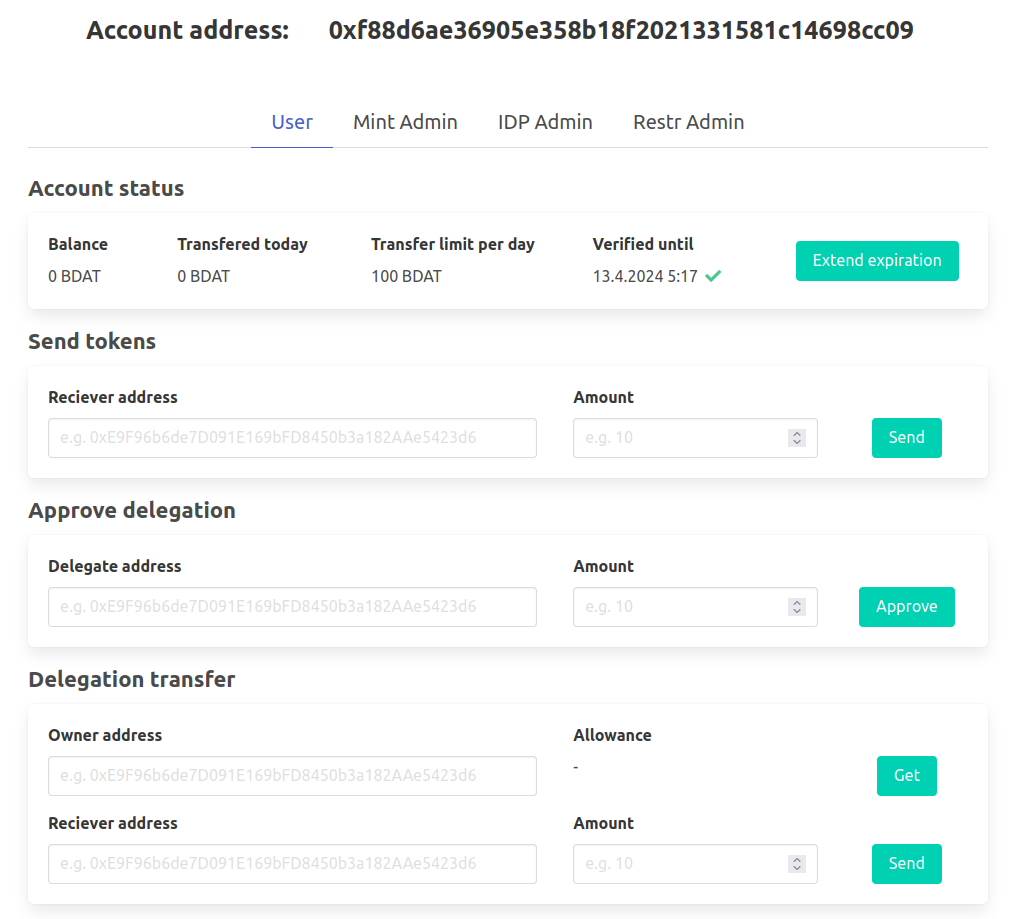
\includegraphics[width=1\linewidth]{images/user-dapp.png}
  \caption{Screenshot of the verified user UI. The user can monitor the status of his account, send tokens, approve delegation, perform delegation, etc.}
  \label{user}
\end{figure*}

\section{Gas Measurements}
The measurement of the gas usage of each function was performed directly in the Truffle tests of the BDAERC20 contract. In the following table, only gas consuming (state modifying) functions are shown. It should also be emphasized that the gas consumption of some functions is strongly dependent on the input parameters. For example, the \texttt{mint} function consumes 126k of gas when minted to a single user, but if minted to 3 users, the gas consumption increases to 194k. The measurement was designed to try to take into account the hardest path in the code (potentially the highest gas usage). Table \ref{table:gas} shows the gas consumption for individual functions.

\begin{table}
\centering
\caption{Gas usage for each (non view/pure) function in the BDAERC20 contract.}
\label{table:gas}
\begin{tabular}{ |l|c| } 
 \noalign{\hrule height 1pt}
 Function & Gas Used \\ 
 \noalign{\hrule height 2pt}
 signAddingIDP & 111111 \\ 
 \hline
 verify & 159954 \\ 
 \hline
  mint & 194370 \\ 
 \hline
  signMint & 111357 \\ 
 \hline
  transfer & 89804 \\ 
 \hline
  approve & 55343 \\ 
 \hline
  transferFrom & 70970 \\ 
 \hline
  signTransferLimitChange & 136671 \\ 
 \hline
  signTMAXChange & 54625 \\ 
 \hline
  signAddingMintingAdmin & 96144 \\ 
 \hline
  signAddingIDPAdmin & 96189 \\ 
 \hline
  signAddingRestrAdmin & 96120 \\ 
 \hline
  signRemovingMintingAdmin & 67757 \\ 
 \hline
  signRemovingIDPAdmin & 67812 \\ 
 \hline
  signRemovingRestrAdmin & 67767 \\ 
 \hline
  signRevoke & 70118 \\ 
 \hline
  signApprove & 55751 \\ 
 \hline
  signRemovingIDP & 62035 \\ 
 \hline
\end{tabular}
\end{table}

\section{Installation instructions for Ubuntu 20.04}
This project (smart contracts and DAPP) was built for and tested on a local blockchain emulated by \textbf{ganache-cli} and managed by \textbf{Truffle} framework (compilation, testing and deployment of smart contracts) and \textbf{MetaMask} wallet (DAPP).

To install the \textbf{Truffle} framework, run:
\begin{itemize}
    \item[] \texttt{sudo apt-get install -y nodejs build-essential}
    \item[] \texttt{sudo npm install -g truffle}
\end{itemize}

To install \textbf{ganache-cli}, run:
\begin{itemize}
    \item[] \texttt{sudo npm install ganache-cli}
\end{itemize}

Next, install the necessary smart contract dependencies using:
\begin{itemize}
    \item[] \texttt{npm install}
\end{itemize}

Install the \textbf{MetaMask} add-on in your browser (tested in Mozilla Firefox 112.0.2 (64-bit) with MetaMask 10.29.0).

Since DAPP needs the address of the deployed contract, this address is hardcoded at the beginning of the \texttt{dapp/script.js} file. In real world conditions, the address of the contract does not change, but when the local blockchain is restarted, the address will change unless \textbf{mnemonic} is specified. Mnemonic is already set inside \texttt{Makefile}. To start the local blockchain, run:
\begin{itemize}
    \item[] \texttt{make blockchain}
\end{itemize}

To deploy the BDAERC20 smart contract, run:
\begin{itemize}
    \item[] \texttt{make deploy}
\end{itemize}

To run DAPP using the \texttt{http.server} Python module, run:
\begin{itemize}
    \item[] \texttt{make run-dapp}
\end{itemize}

DAPP is now available through a web browser at \url{http://localhost:8000}.

To run Truffle tests and/or gas measurements, run:
\begin{itemize}
    \item[] \texttt{truffle test}
\end{itemize}


\newpage
\bibliography{BDA-bib} 
\bibliographystyle{bib-styles/czplain}

\end{document}
